\documentclass{beamer}
\usepackage{graphicx}

\usepackage{amsmath}
\usepackage{hyperref}
\usepackage{multicol}
\usetheme{Warsaw}
\usepackage{color}
\title{Tutorial 7}
\author{CB2200 Business Statistics, YANG Yihang}
\date{\today}

\begin{document}
\titlepage
\begin{frame}
	\frametitle{Intended Learning Outcomes}
	After this tutorial, you may know how to 
	\begin{itemize}
		\item utilize $Z$ table and $t$ table
		\item calculate the C.I(Confidence interval) with respect to a confidence level.
		\item interpret the confidence interval
		\end{itemize}
	\end{frame}
\begin{frame}
	\frametitle{Recap}
	\begin{figure}
		\begin{center}
			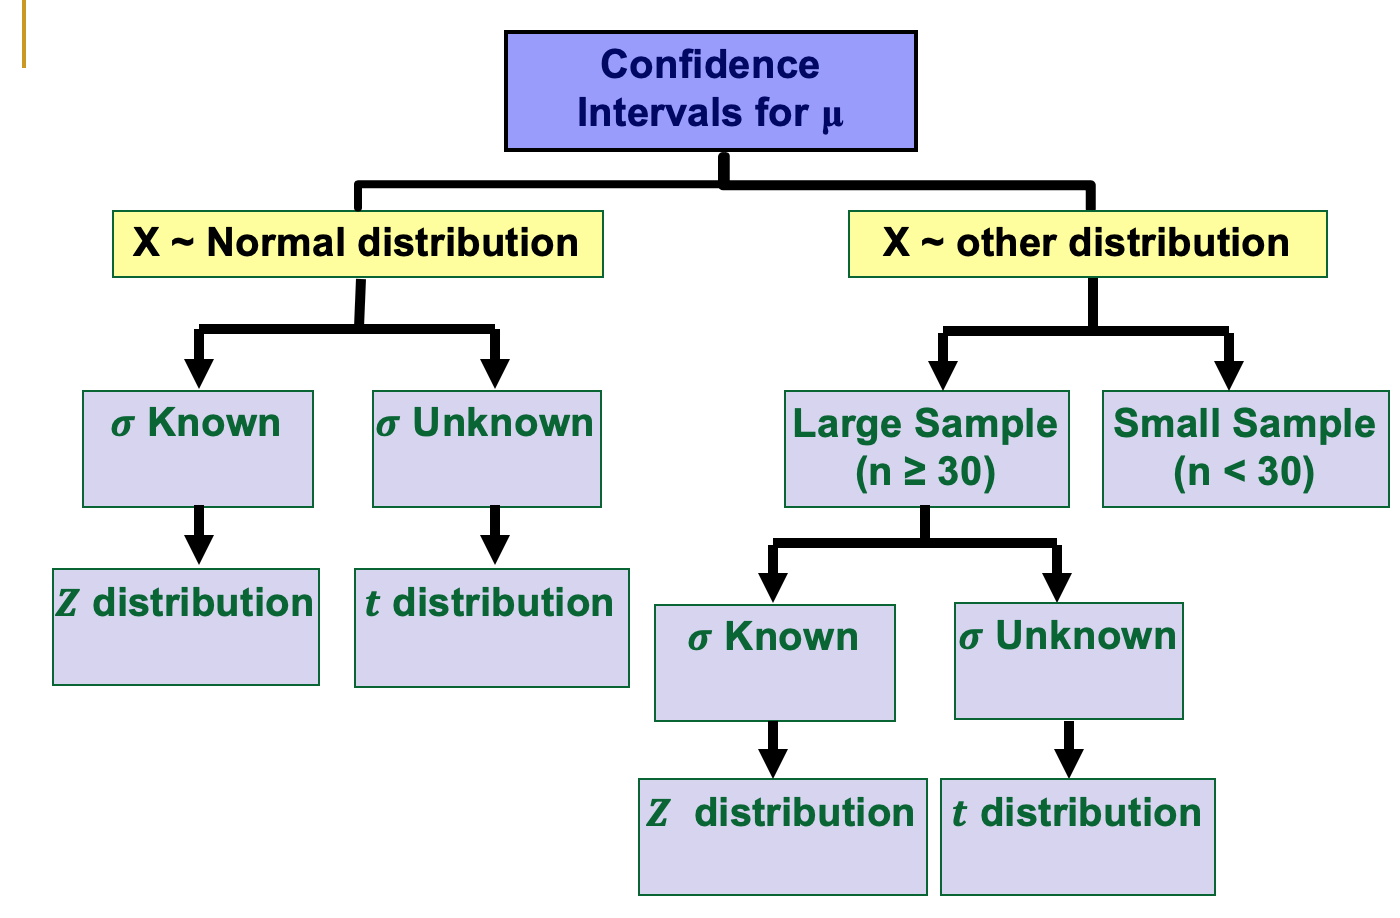
\includegraphics[scale=0.40]{recap1.png}
		\end{center}
	\end{figure}
\end{frame}
\begin{frame}
\frametitle{Conditions of Utilizing Z table}
\begin{figure}
	\begin{center}
		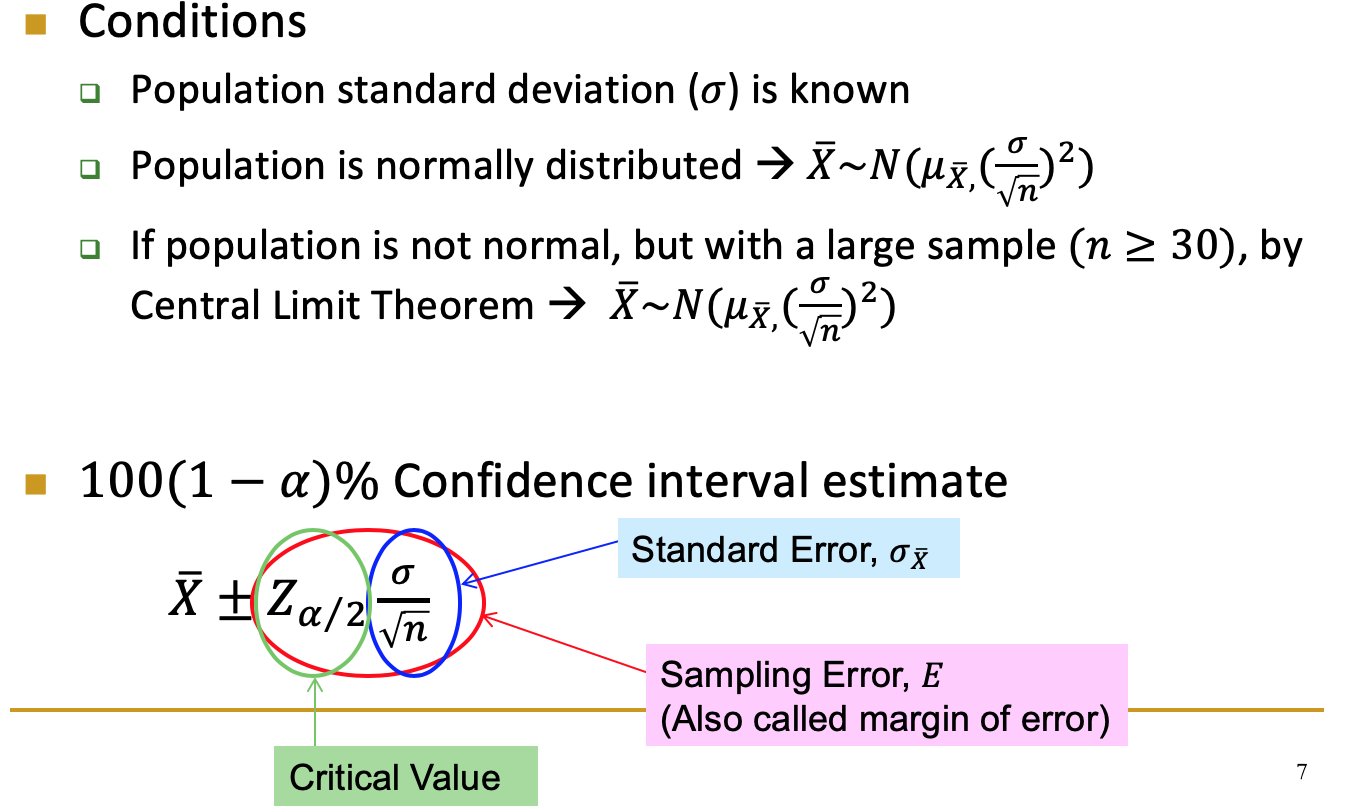
\includegraphics[scale=0.40]{recap2.png}
	\end{center}
\end{figure}
\end{frame}
\begin{frame}
\frametitle{Conditions of Utilizing t table}
\begin{figure}
	\begin{center}
		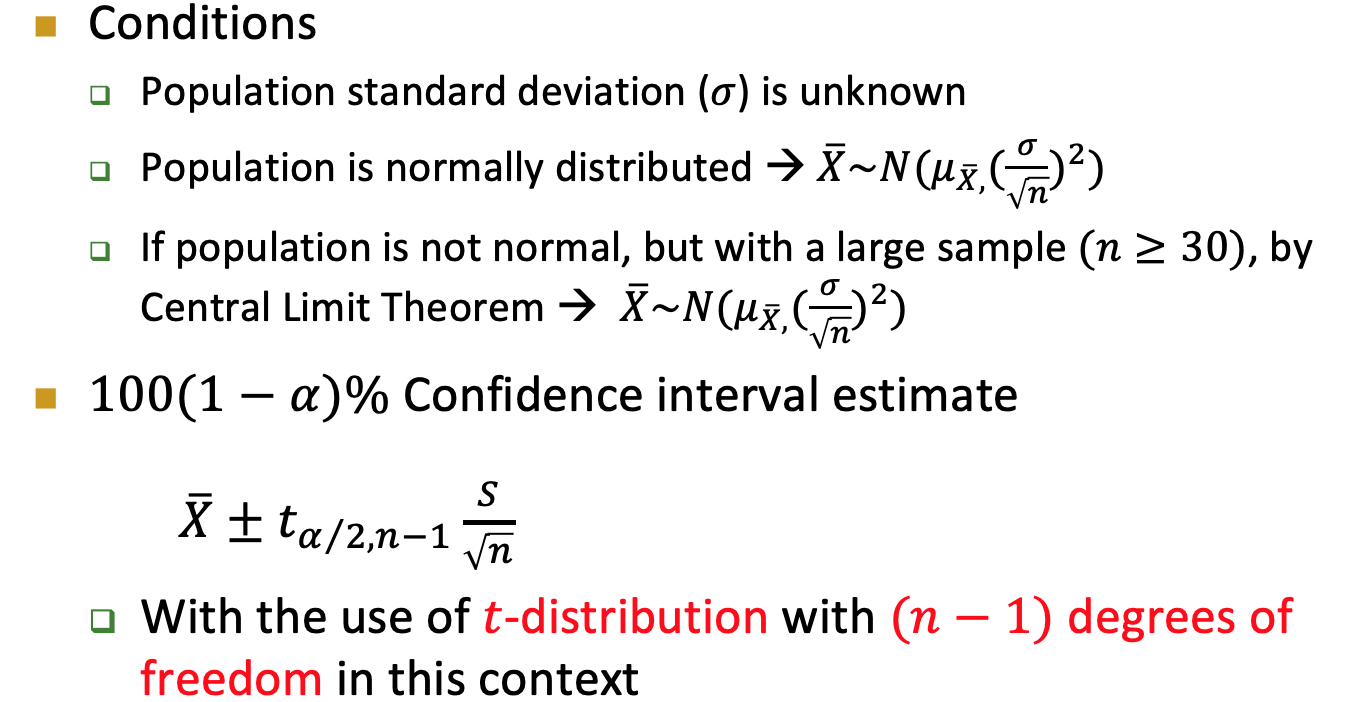
\includegraphics[scale=0.40]{recap3.png}
	\end{center}
\end{figure}
\end{frame}

\begin{frame}
\frametitle{Question 1}

\begin{figure}
	\begin{center}
		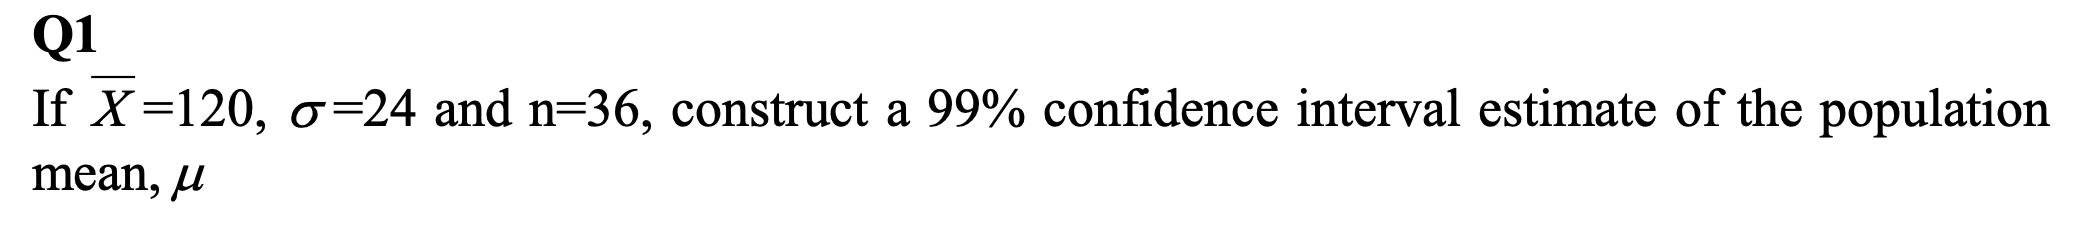
\includegraphics[scale=0.30]{Q1.png}
	\end{center}
\end{figure}
\end{frame}
\begin{frame}
\frametitle{Question 1}
\begin{figure}
	\begin{center}
		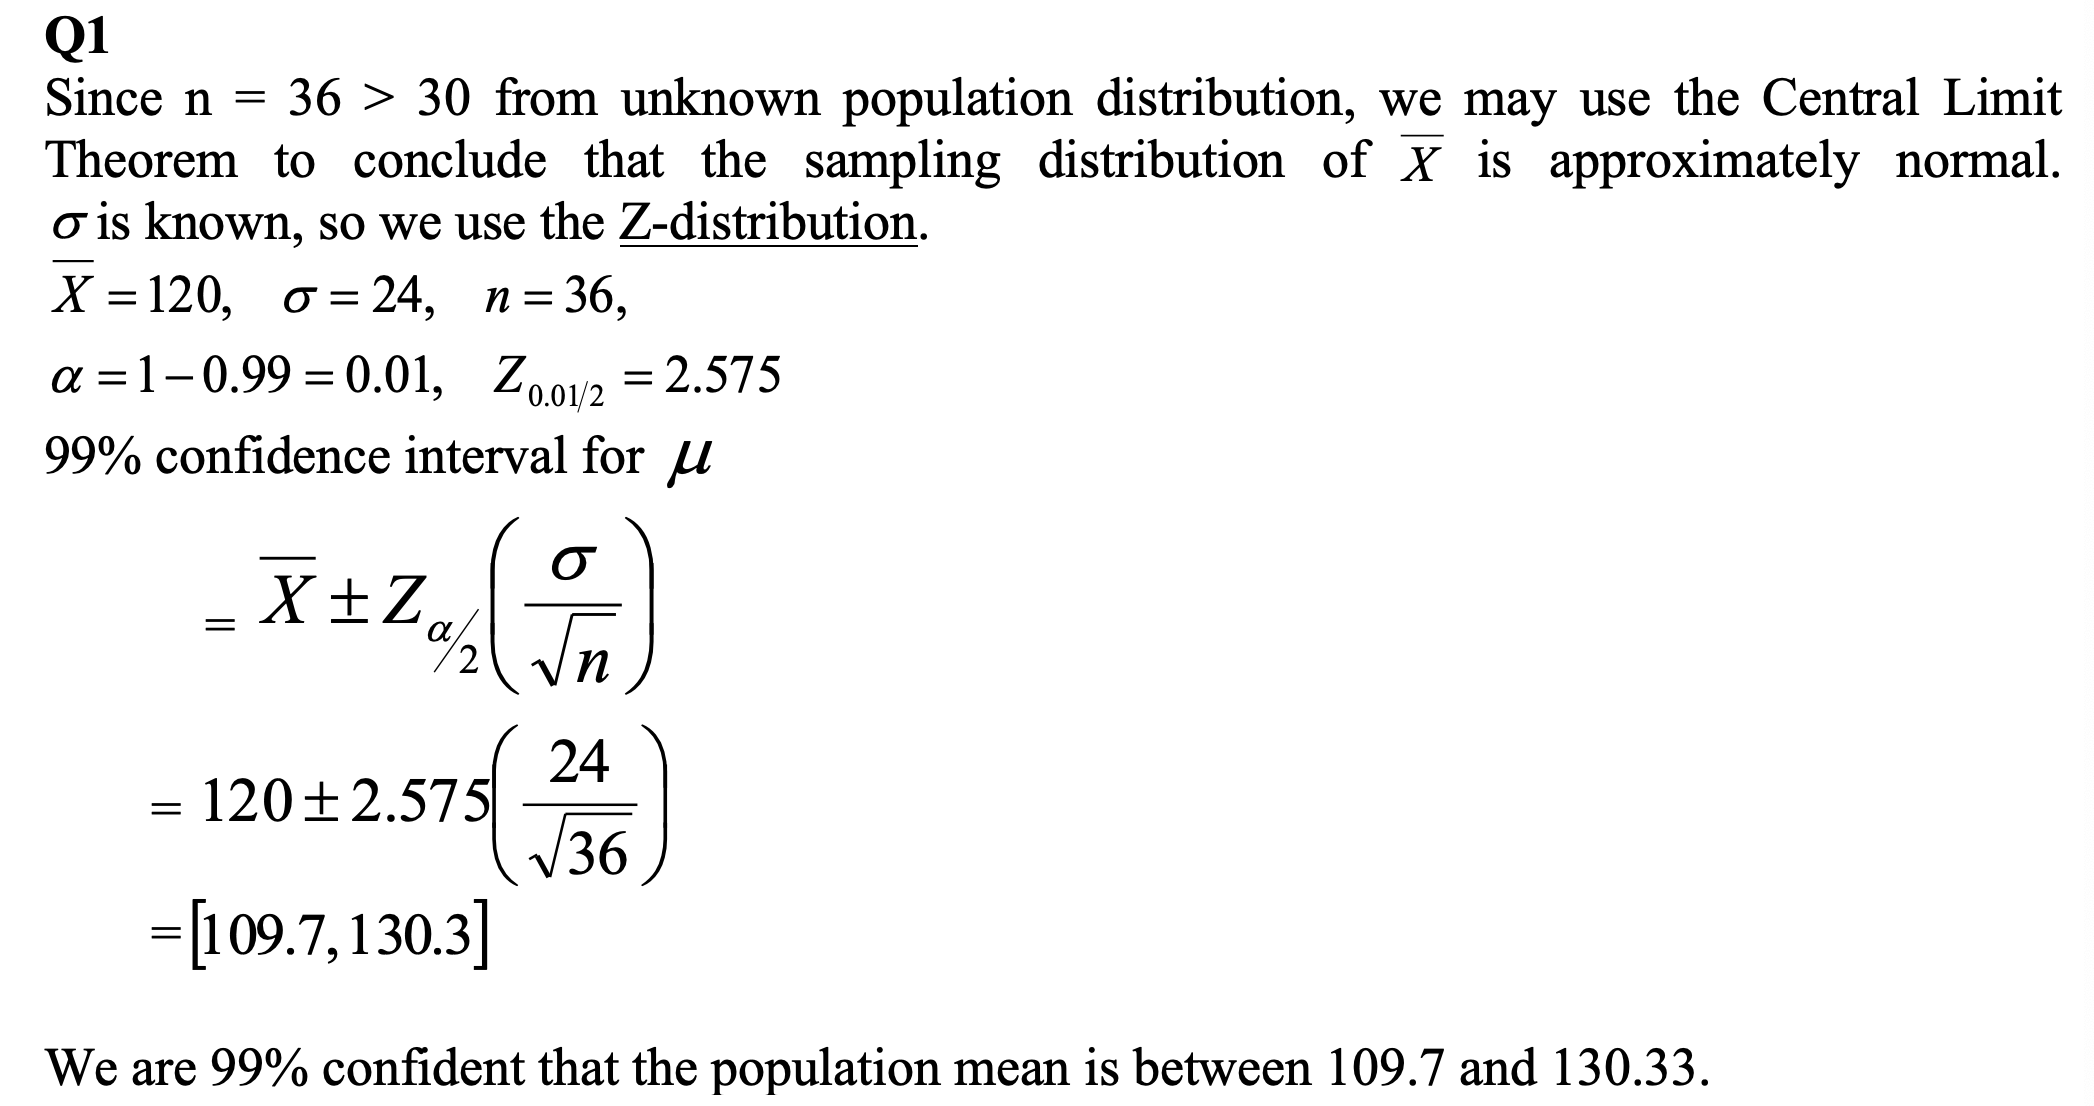
\includegraphics[scale=0.30]{Q1_sol.png}
	\end{center}
\end{figure}
\end{frame}

\begin{frame}
\frametitle{Question 2}

\begin{figure}
	\begin{center}
		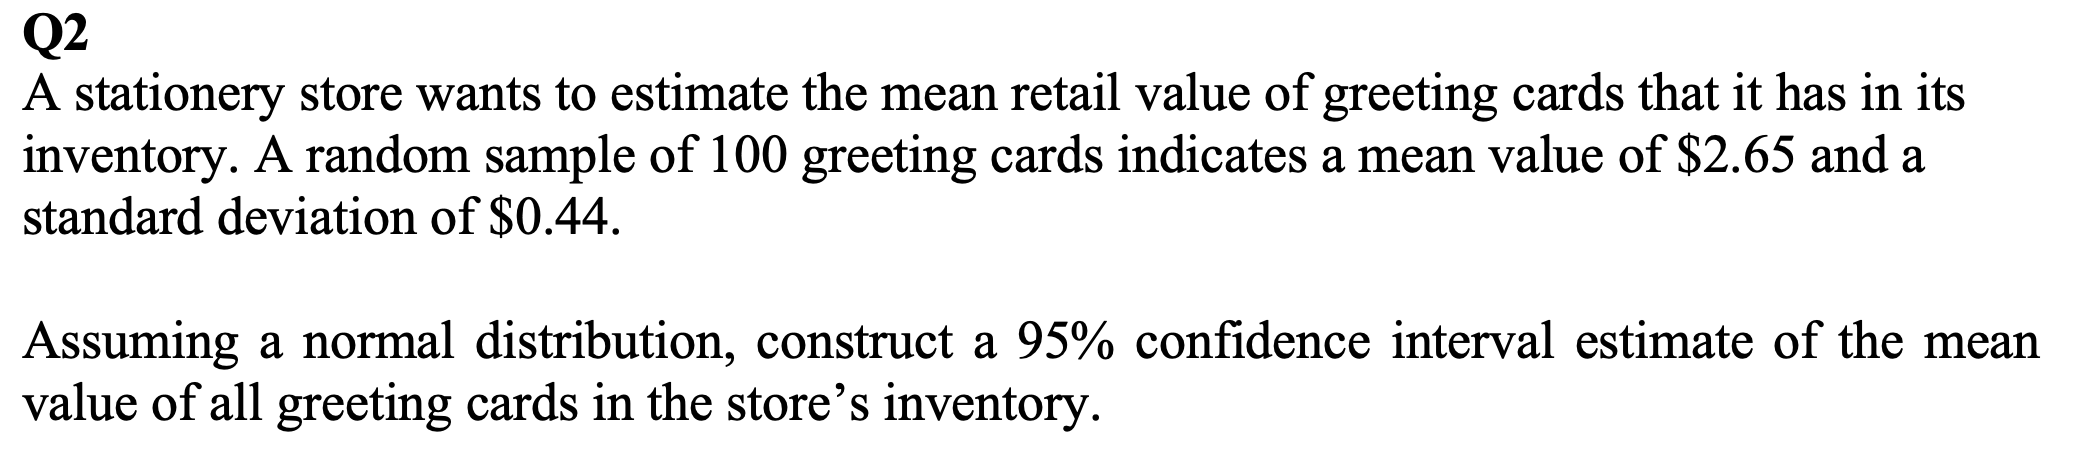
\includegraphics[scale=0.30]{Q2.png}
	\end{center}
\end{figure}
\end{frame}
\begin{frame}
\frametitle{Question 2}
\begin{figure}
\begin{center}
	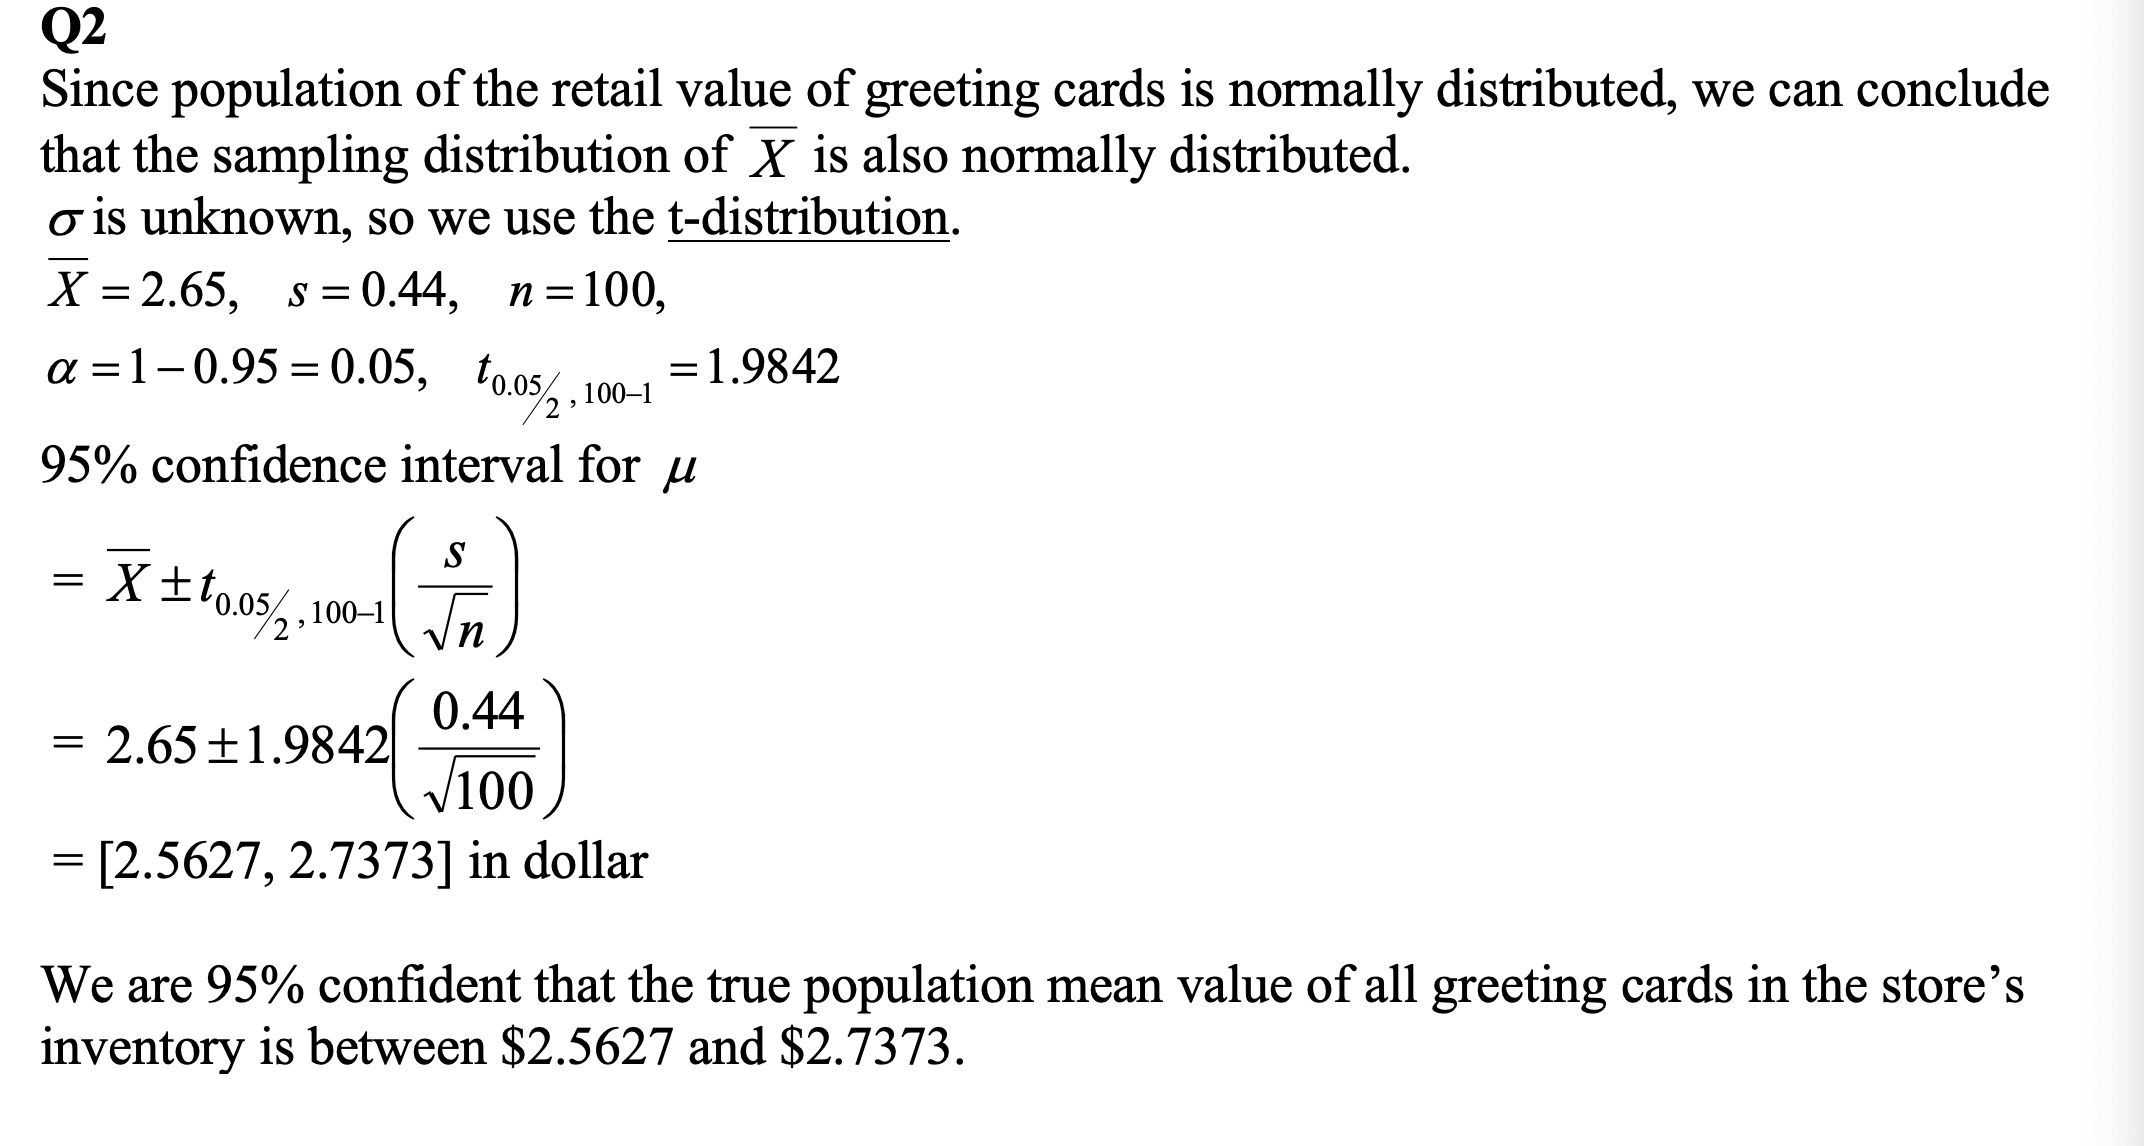
\includegraphics[scale=0.30]{Q2_sol.png}
\end{center}
\end{figure}
\end{frame}
\begin{frame}
\frametitle{Question 3}
\begin{figure}
\begin{center}
	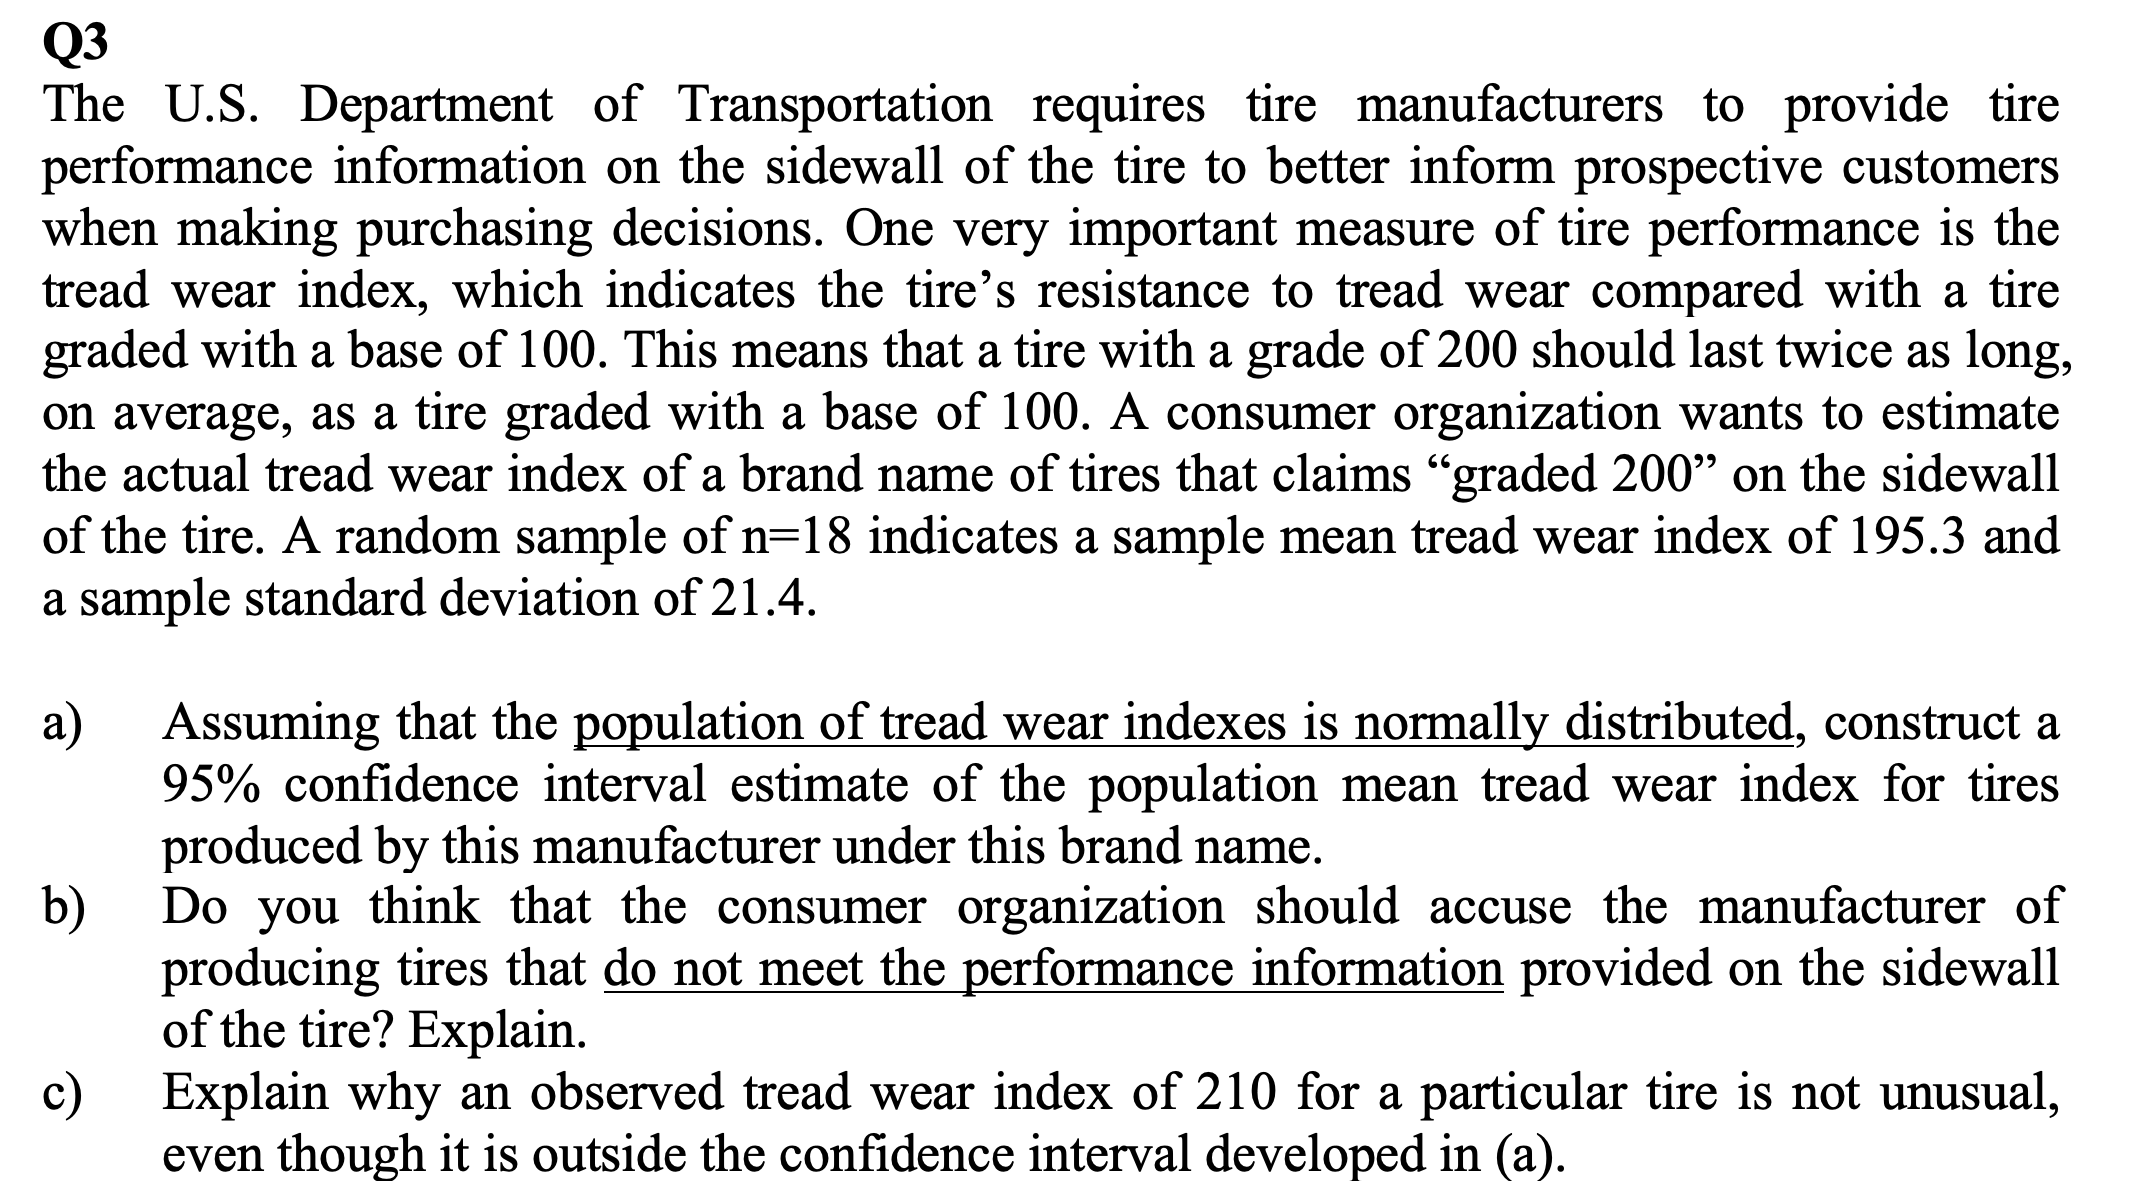
\includegraphics[scale=0.30]{Q3.png}
\end{center}
\end{figure}
\end{frame}
\begin{frame}
\frametitle{Question 3}

\begin{figure}
	\begin{center}
		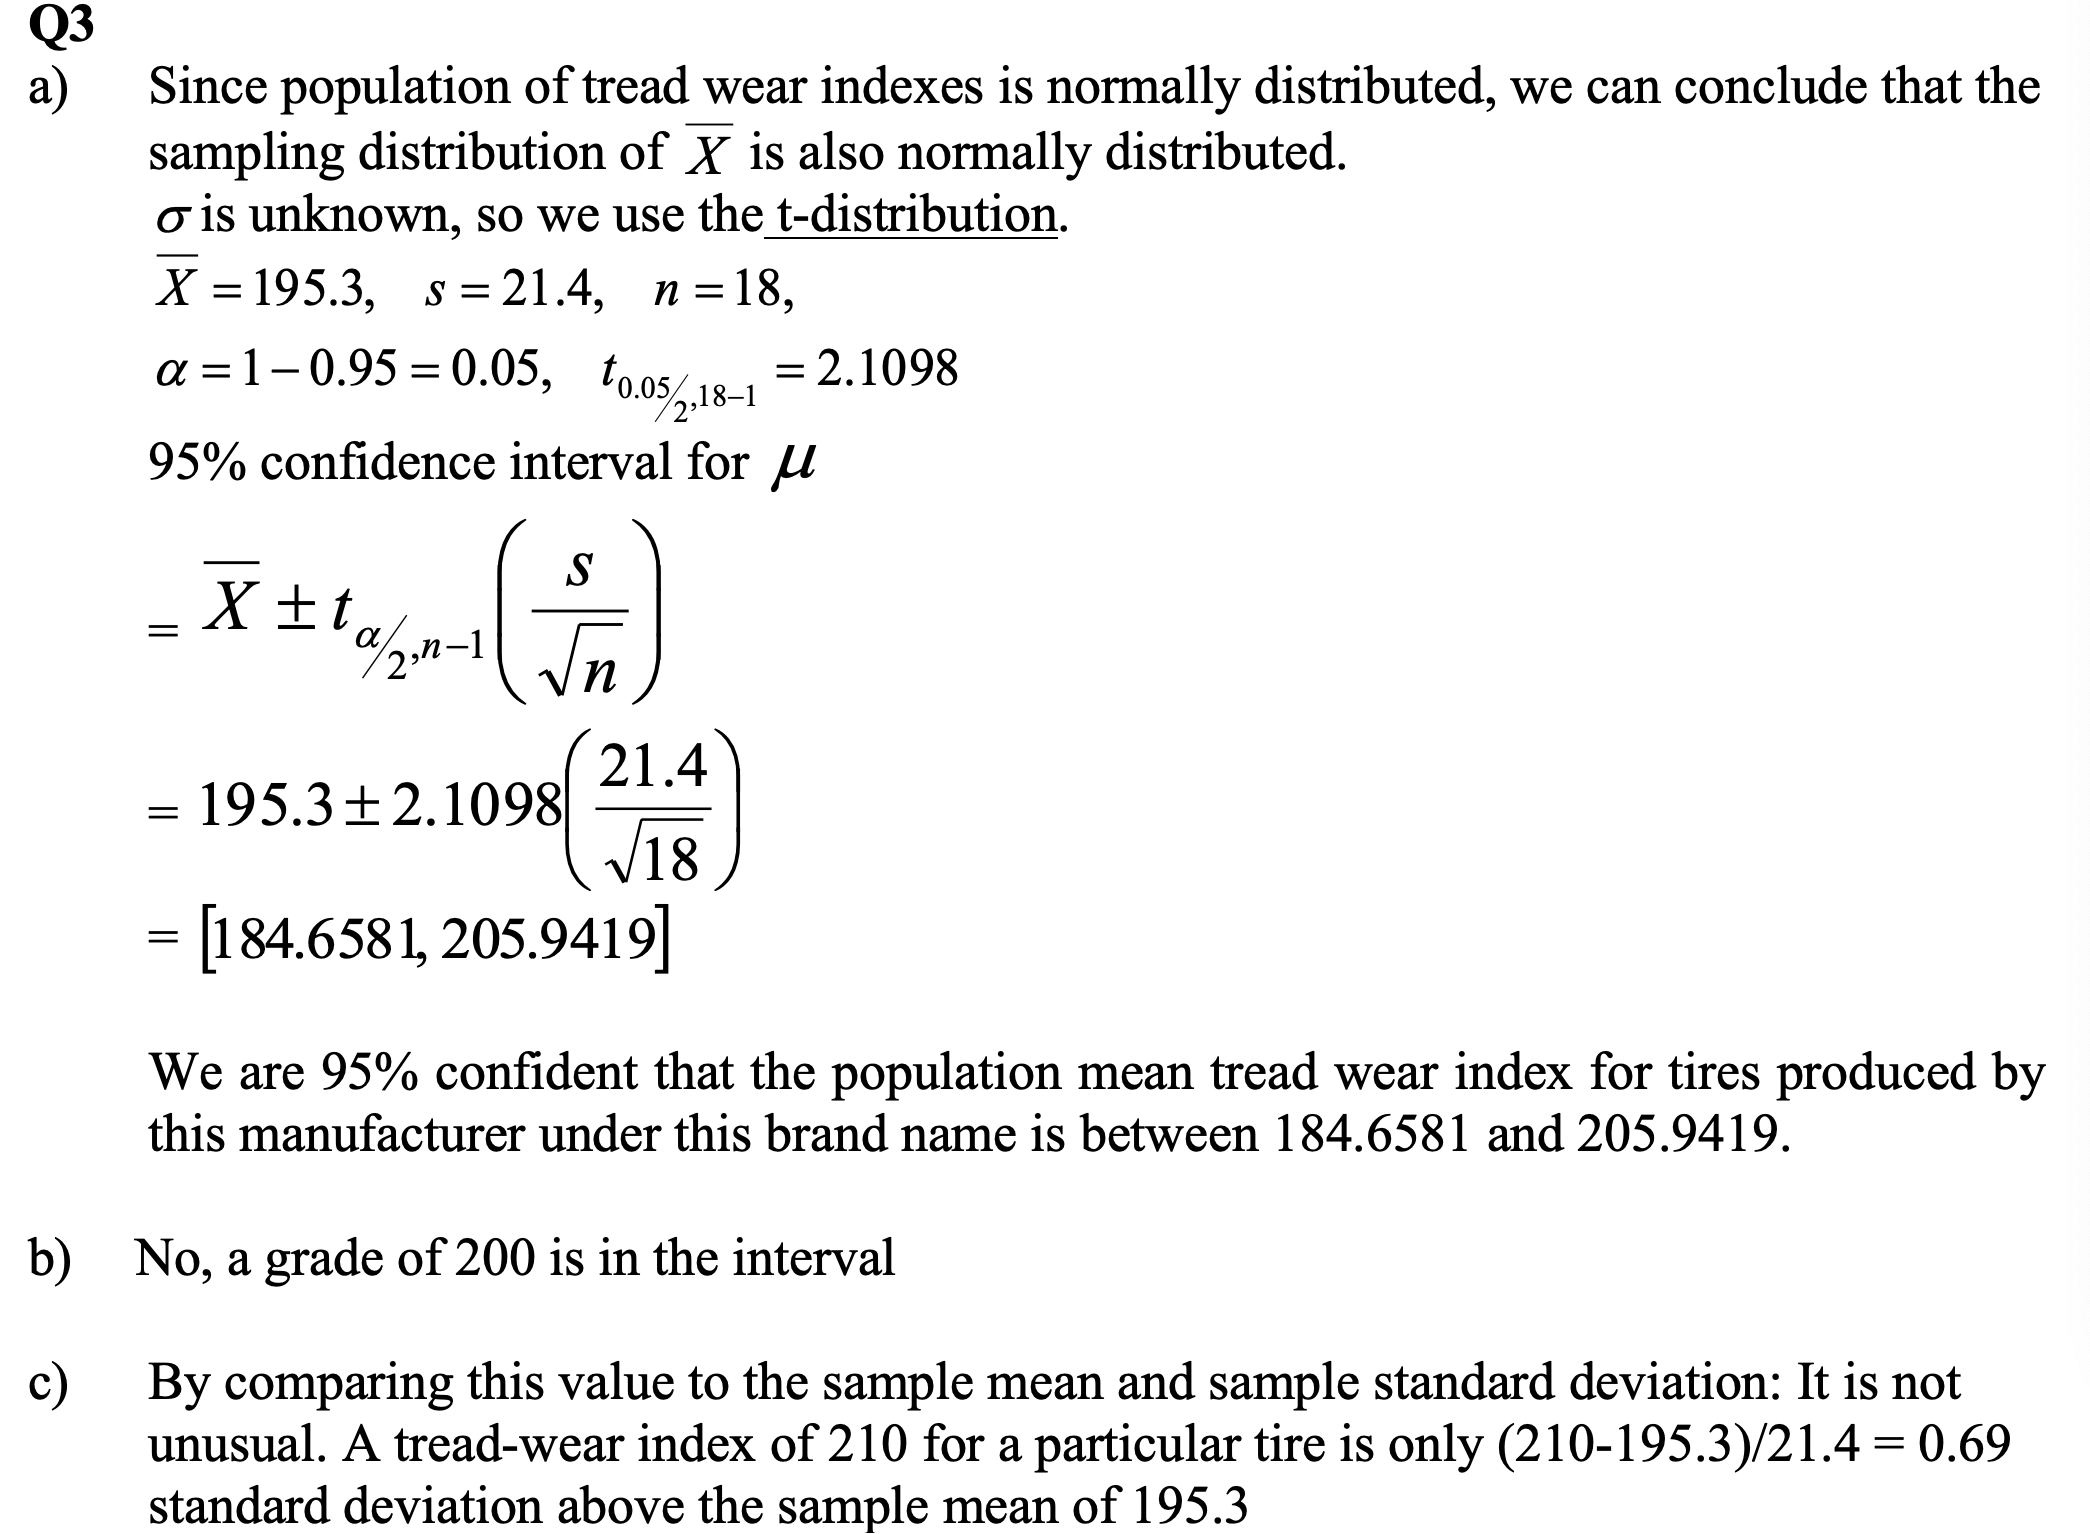
\includegraphics[scale=0.30]{Q3_sol.png}
	\end{center}
\end{figure}
\end{frame}
\begin{frame}
\frametitle{Question 6}

\begin{figure}
	\begin{center}
		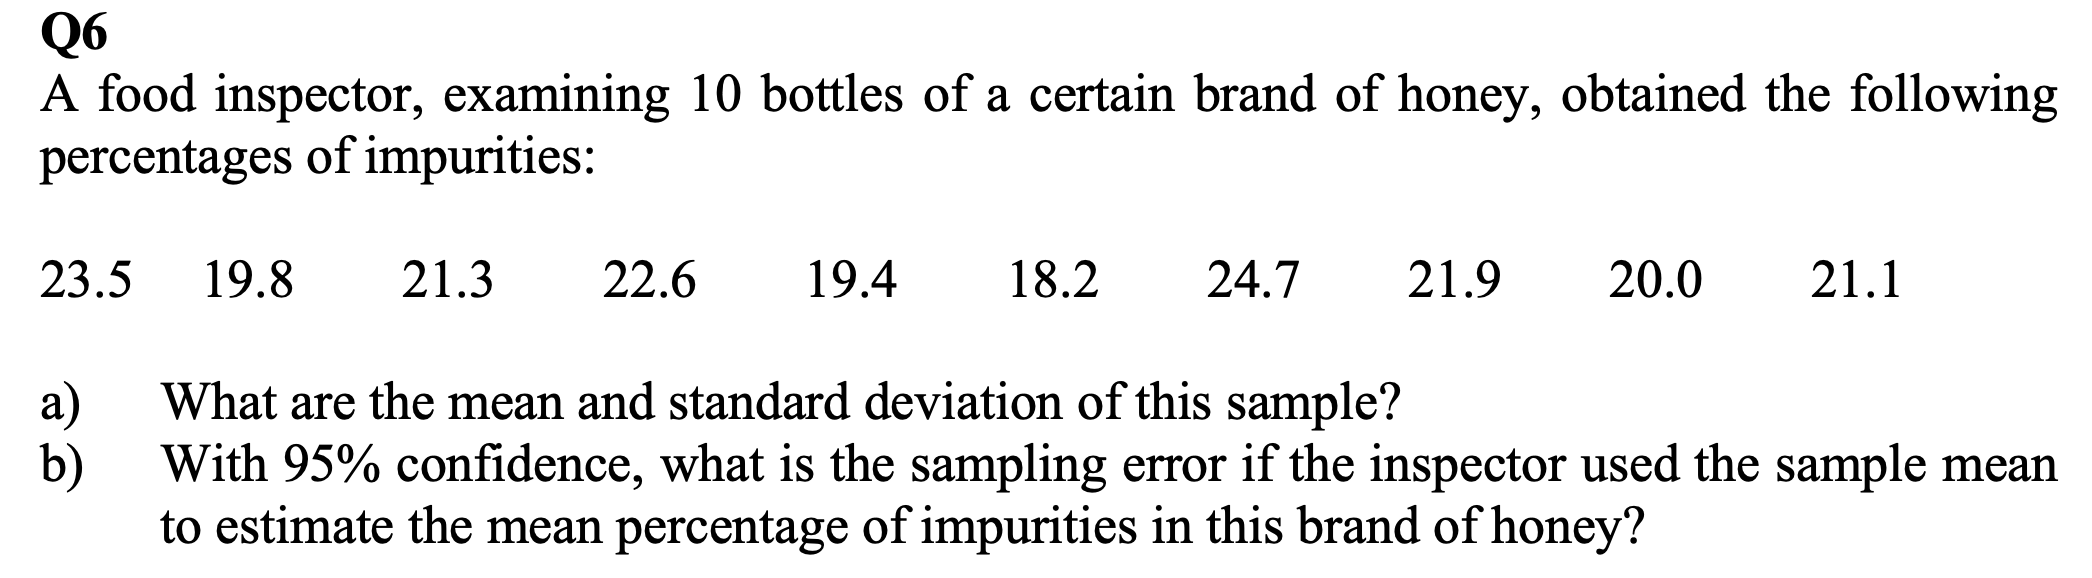
\includegraphics[scale=0.30]{Q6.png}
	\end{center}
\end{figure}
\end{frame}
\begin{frame}
\frametitle{Question 6}
\begin{figure}
\begin{center}
	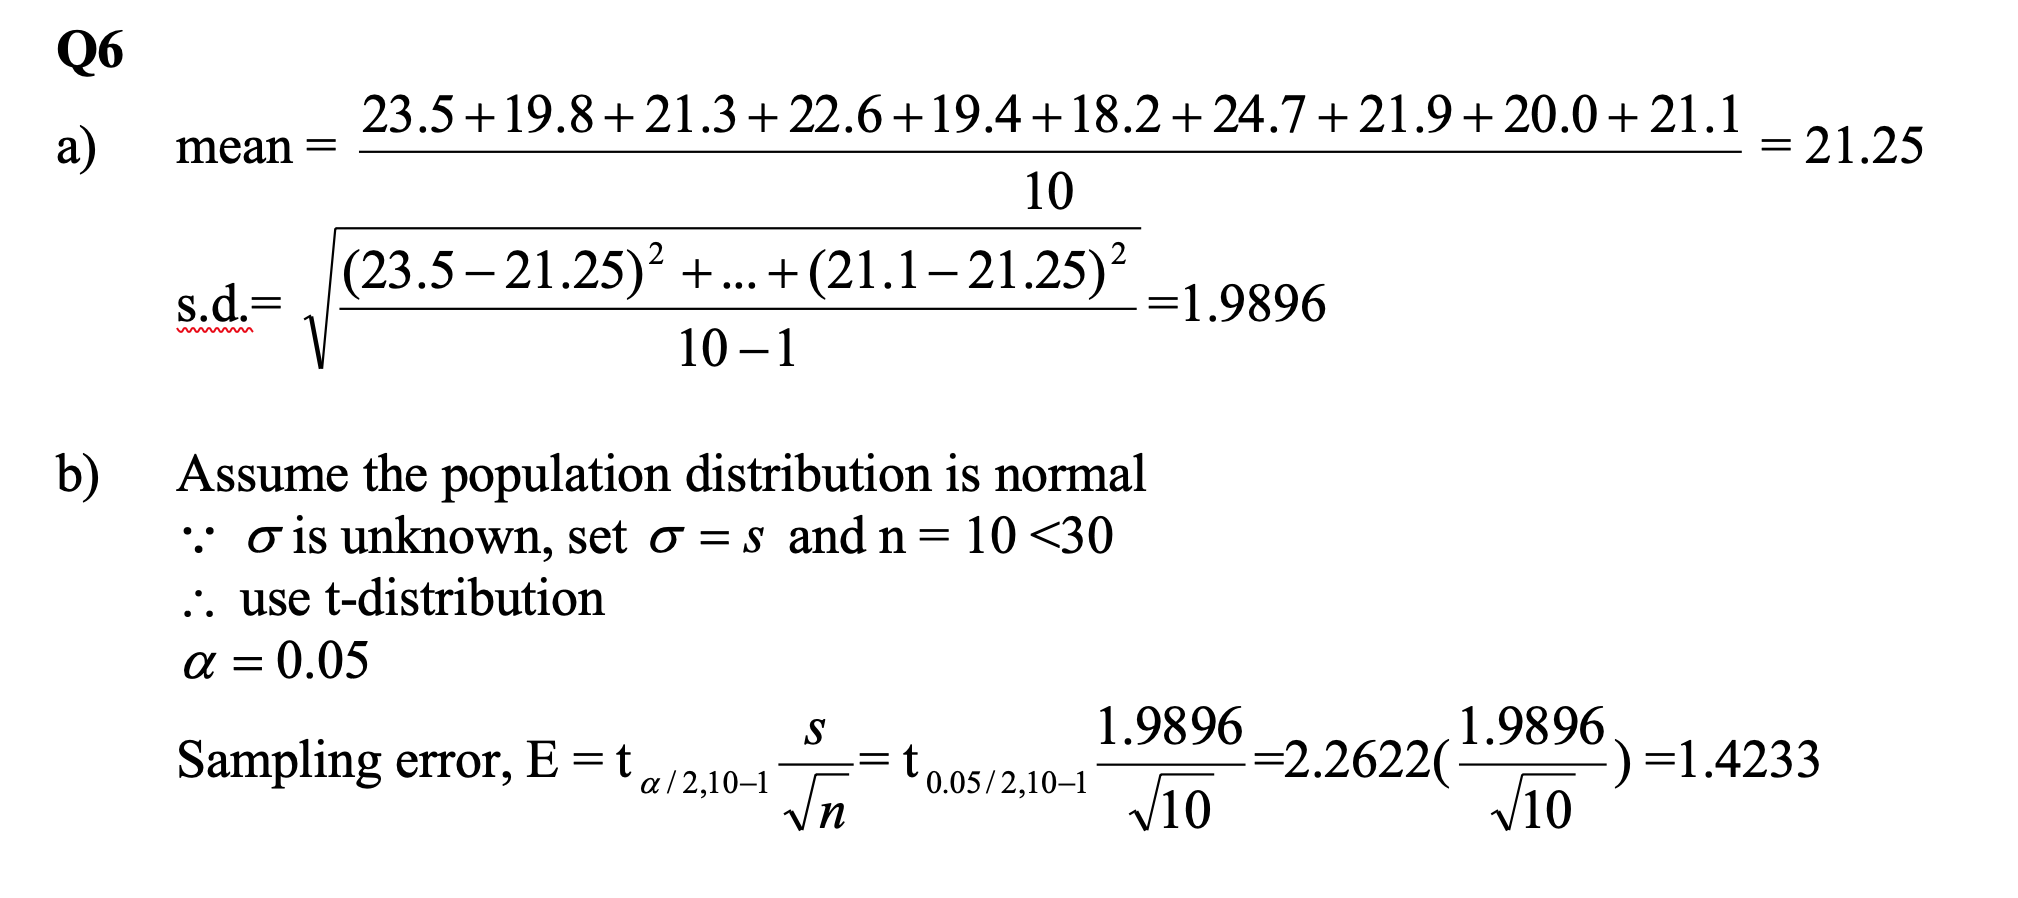
\includegraphics[scale=0.30]{Q6_sol.png}
\end{center}
\end{figure}
\end{frame}
\begin{frame}
\frametitle{Question 7}

\begin{figure}
	\begin{center}
		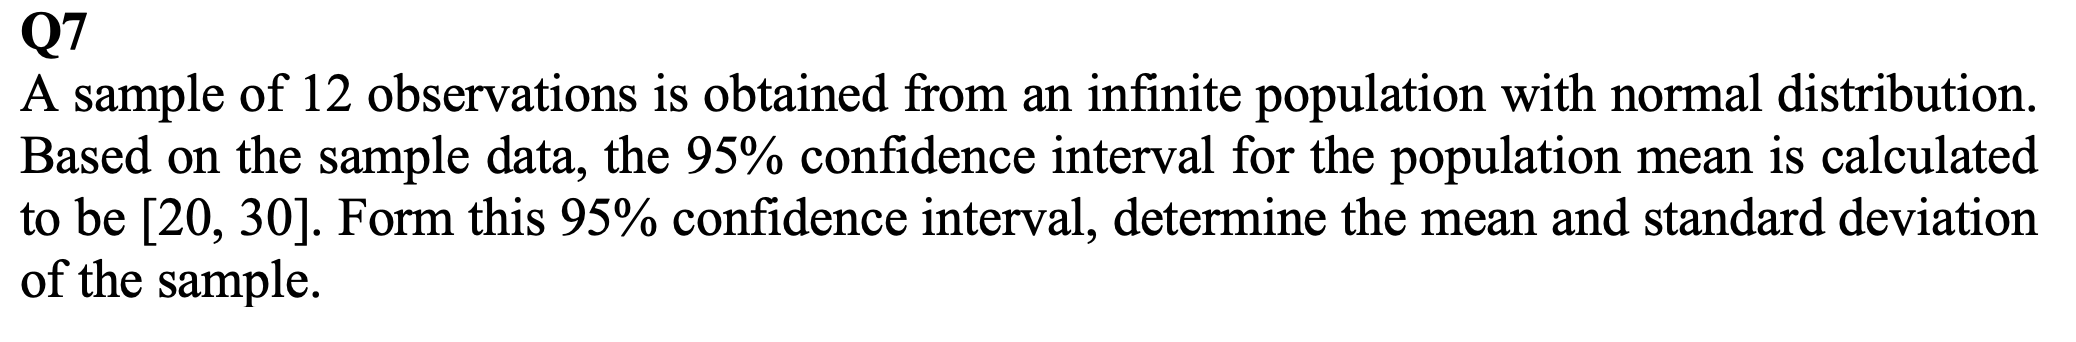
\includegraphics[scale=0.30]{Q7.png}
	\end{center}
\end{figure}
\end{frame}
\begin{frame}
\frametitle{Question 7}
\begin{figure}
\begin{center}
	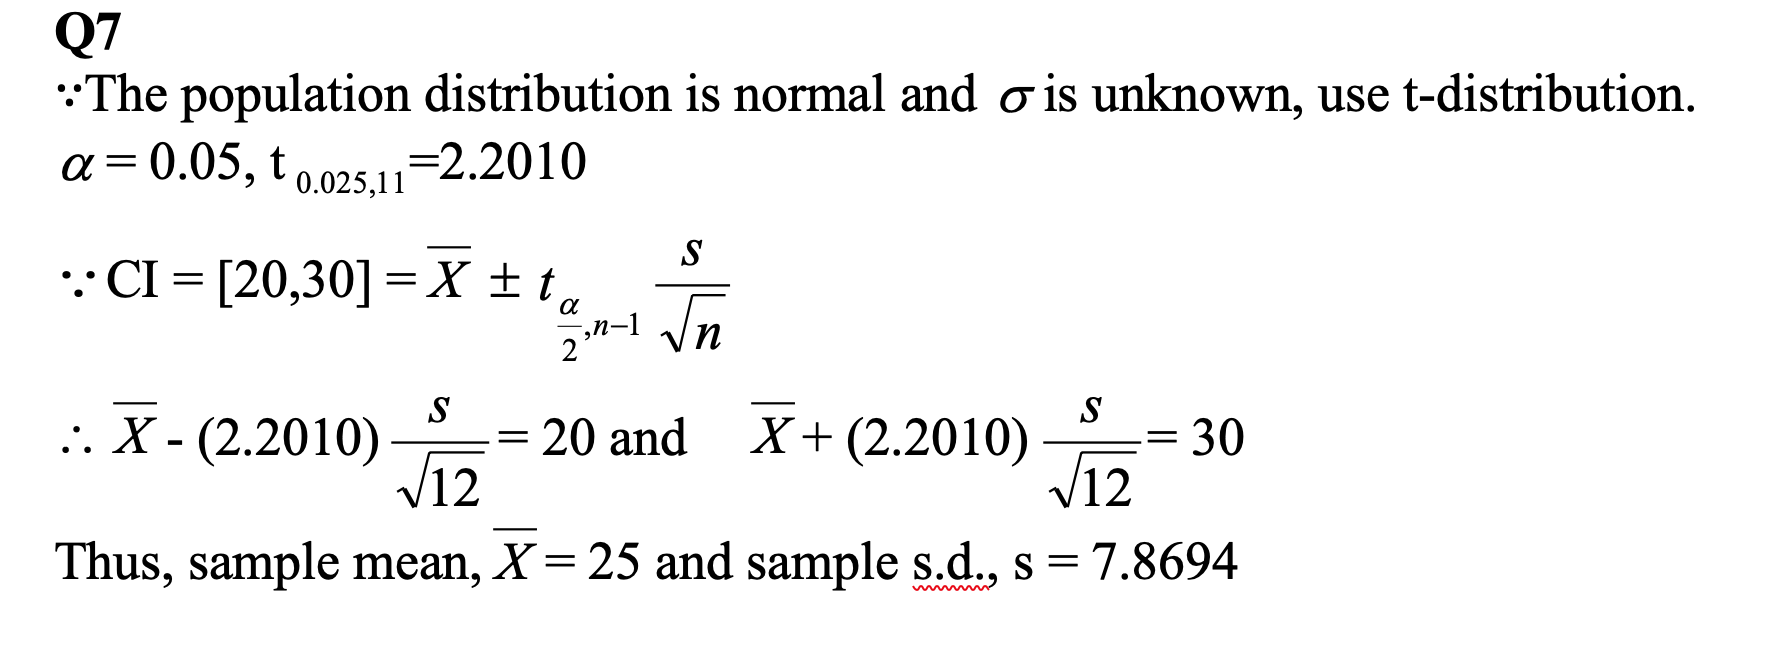
\includegraphics[scale=0.35]{Q7_sol.png}
\end{center}
\end{figure}
\end{frame}

\end{document}

